% GHOST system model with the real intermediate tensors of one request
% (ResNet-20, split after block 3, rho = 10, CIFAR-10 test image 1398; layer blocks.0.conv1 shown),
% produced by ghost2/fig_tensors.py. Drawn at IEEE \textwidth (7.16in).
\documentclass[tikz,border=1pt,10pt]{standalone}
\usepackage[T1]{fontenc}
\usepackage{mathptmx}
\usepackage{courier}
\usepackage{graphicx}
\usetikzlibrary{arrows.meta,calc}
\definecolor{ink}{HTML}{1A1A1A}
\definecolor{dark}{HTML}{263238}
\definecolor{teeC}{HTML}{2E7D32}\definecolor{teeF}{HTML}{EDF6EE}
\definecolor{reeC}{HTML}{C62828}\definecolor{reeF}{HTML}{FCEDED}
\definecolor{clC}{HTML}{1565C0}\definecolor{clF}{HTML}{EAF2FB}
\definecolor{setC}{HTML}{6A1B9A}\definecolor{setF}{HTML}{F4EEF8}
\definecolor{devC}{HTML}{37474F}
\definecolor{acc}{HTML}{E65100}
\definecolor{bar}{HTML}{4A6FA5}
\def\TokHex{e1817c66}
\def\CtHex{d06c51cc}
\def\PredClass{Horse}
\def\ProbList{0.056,0.000,0.013,0.041,0.001,0.066,0.000,0.813,0.008,0.002}
\def\WRows{16}\def\WtRows{20}

\graphicspath{{arch_assets/}}
\tikzset{
  >={Stealth[length=1.9mm,width=1.5mm]},
  font=\scriptsize, every node/.style={text=ink},
  zone/.style={draw=#1,line width=1pt,rounded corners=2.5pt},
  tab/.style={fill=#1,text=white,font=\footnotesize\bfseries,inner xsep=3pt,inner ysep=2pt,rounded corners=1.5pt},
  vtab/.style={fill=#1,text=white,font=\footnotesize\bfseries,rotate=90,inner xsep=3pt,inner ysep=2pt},
  ttl/.style={align=center,inner sep=0.8pt,font=\scriptsize},
  f/.style={->,draw=dark,line width=0.8pt},
  fo/.style={->,draw=setC,line width=0.8pt,dash pattern=on 3pt off 1.8pt},
  bridge/.style={preaction={draw=white,line width=3.2pt,-}},
  n/.style={circle,draw=dark,line width=0.7pt,fill=white,text=dark,font=\scriptsize\bfseries,inner sep=0pt,minimum size=3.6mm},
  lab/.style={font=\scriptsize,inner sep=1pt},
}
% stack of four channel maps: front tile 0.82cm, offset 0.1cm, centred at (#1,#2)
\newcommand{\fstack}[3]{%
  \foreach \k in {3,2,1,0}{%
    \node[inner sep=0pt,anchor=south west,draw=ink,line width=0.3pt]
      at ({#1-0.56+\k*0.1},{#2-0.56+\k*0.1}) {\includegraphics[width=0.82cm]{#3\k}};}}
\newcommand{\tile}[4]{\node[inner sep=0pt,draw=ink,line width=0.4pt] at (#1,#2) {\includegraphics[width=#4]{#3}};}
\newcommand{\inset}[3]{\node[inner sep=0pt,draw=white,line width=1pt] at (#1,#2) {\includegraphics[width=0.42cm]{#3}};
  \draw[ink,line width=0.4pt] ($(#1,#2)+(-0.21,-0.21)$) rectangle ++(0.42,0.42);}
\newcommand{\padlock}[3][1]{%
  \begin{scope}[shift={(#2,#3)},scale=#1]
   \draw[dark,line width=1.2pt] (-0.1,0.09) -- (-0.1,0.18) arc (180:0:0.1) -- (0.1,0.09);
   \fill[dark,rounded corners=1pt] (-0.17,-0.15) rectangle (0.17,0.11);
   \fill[white] (0,-0.02) circle (0.04);
  \end{scope}}
\newcommand{\shield}[3]{% x y colour
  \begin{scope}[shift={(#1,#2)}]
  \fill[#3] (0,0.42) .. controls (0.2,0.34) .. (0.32,0.34) -- (0.32,0.04) .. controls (0.32,-0.23) .. (0,-0.38)
              .. controls (-0.32,-0.23) .. (-0.32,0.04) -- (-0.32,0.34) .. controls (-0.2,0.34) .. cycle;
  \draw[white,line width=1.4pt,line cap=round,line join=round] (-0.15,0.0) -- (-0.03,-0.12) -- (0.17,0.15);
  \end{scope}}
\newcommand{\cuboid}[5]{%
  \fill[#5,draw=dark,line width=0.5pt] (#1,#2-#4/2) rectangle ++(#3,#4);
  \fill[#5!70!black,draw=dark,line width=0.5pt] (#1,#2+#4/2) -- ++(0.1,0.1) -- ++(#3,0) -- ++(-0.1,-0.1) -- cycle;
  \fill[#5!85!black,draw=dark,line width=0.5pt] (#1+#3,#2-#4/2) -- ++(0.1,0.1) -- ++(0,#4) -- ++(-0.1,-0.1) -- cycle;}
\begin{document}
\begin{tikzpicture}
% ================================================================= zones
\draw[zone=devC] (0,2.95) rectangle (1.95,9.45);
\node[tab=devC] at (0.975,9.45) {Client};
\draw[zone=devC] (2.1,2.95) rectangle (15.8,9.45);
\node[tab=devC] at (8.95,9.45) {Edge Device};
\draw[zone=teeC,fill=teeF] (2.25,5.95) rectangle (15.65,9.25);
\fill[teeC] (2.25,5.95) rectangle (2.65,9.25);
\node[vtab=teeC] at (2.45,7.6) {TEE (Trusted)};
\draw[zone=teeC] (2.25,5.95) rectangle (15.65,9.25);
\draw[zone=reeC,fill=reeF,dash pattern=on 4pt off 2pt] (4.75,3.1) rectangle (15.65,5.75);
\fill[reeC] (4.75,3.1) rectangle (5.15,5.75);
\node[vtab=reeC] at (4.95,4.425) {REE (Adversary)};
\draw[zone=reeC,dash pattern=on 4pt off 2pt] (4.75,3.1) rectangle (15.65,5.75);
\draw[zone=clC,fill=clF] (15.95,2.95) rectangle (18.3,9.45);
\node[tab=clC] at (17.125,9.45) {Cloud Service};
\draw[zone=setC,fill=setF] (0,0.45) rectangle (18.3,2.5);
\fill[setC] (0,0.45) rectangle (0.4,2.5);
\node[vtab=setC] at (0.2,1.475) {Setup};
\draw[zone=setC] (0,0.45) rectangle (18.3,2.5);

% ================================================================= client
\node[ttl,anchor=south,font=\footnotesize] at (0.975,8.08) {Input and Token};
\tile{0.975}{7.45}{input}{1.1cm}
\node[draw=dark,fill=white,rounded corners=2pt,line width=0.6pt,font=\scriptsize\ttfamily\bfseries,inner sep=1.8pt] (tok) at (0.975,6.5) {\TokHex};
\draw[dark,line width=0.6pt] (0.975,6.9) -- (tok.north);
\node[ttl,anchor=south,font=\footnotesize] at (0.975,5.72) {Prediction};
\foreach \c [count=\i from 0] in {plane,car,bird,cat,deer,dog,frog,horse,ship,truck}{%
  \pgfmathsetmacro{\p}{{\ProbList}[\i]}
  \pgfmathsetmacro{\yy}{5.55-\i*0.215}
  \node[lab,anchor=east] at (0.68,\yy) {\c};
  \ifnum\i=7
    \fill[acc] (0.72,\yy-0.08) rectangle ++({0.85*\p},0.16);
    \node[lab,anchor=west,font=\scriptsize\bfseries] at ({0.72+0.85*\p},\yy) {\pgfmathprintnumber[fixed,precision=2]{\p}};
  \else
    \fill[bar] (0.72,\yy-0.08) rectangle ++({max(0.85*\p,0.015)},0.16);
  \fi}
\draw[dark,line width=0.6pt] (0.72,5.67) -- (0.72,3.5);

% ================================================================= TEE (online)
\def\ty{7.45}
\foreach \x/\t in {3.55/{Token and\\Budget Check},4.98/{First\\Convolution},6.41/{Channel\\Mixing},7.84/{One-Time\\Masking},
  9.27/{Precomputed\\Correction},10.7/{Correction\\Removal},12.13/{Unmixing and\\Decoy Removal},13.56/{Bias and\\Activation},14.99/{Feature\\Encryption}}
  {\node[ttl,anchor=north] at (\x,8.82) {\t};}
\shield{3.55}{7.62}{teeC}
\foreach \j in {0,...,7}{\ifnum\j<3 \fill[teeC] \else \draw[teeC,line width=0.45pt,fill=white] \fi ({2.97+\j*0.15},6.92) rectangle ++(0.11,0.17);}
\fstack{4.98}{\ty}{a}
\fstack{6.41}{\ty}{Ba}   \inset{6.86}{7.02}{B}
\fstack{7.84}{\ty}{R}
\fstack{9.27}{\ty}{M}
\fstack{10.7}{\ty}{z}
\fstack{12.13}{\ty}{u}   \inset{12.58}{7.02}{A}
\fstack{13.56}{\ty}{act}
\tile{14.99}{\ty}{ct}{0.85cm}
\padlock[0.9]{15.3}{7.82}
\foreach \a/\b in {4.17/4.42,5.54/5.85,6.97/7.28,8.4/8.71,9.83/10.14,11.26/11.57,12.69/13.0,14.12/14.56}
  \draw[f] (\a,\ty) -- (\b,\ty);
\draw[f] (2.1,\ty) ++(-0.585,0) -- node[pos=0.12,n,above=1.5pt]{1} (2.92,\ty);

% ================================================================= REE
\def\ry{4.6}
\tile{6.41}{4.45}{Wt}{0.95cm}
\node[ttl,anchor=south] at (6.41,4.96) {Obfuscated Weights};
\fstack{7.84}{\ry}{xt}
\node[ttl,anchor=north] at (7.84,3.97) {Masked Activation};
\begin{scope}[shift={(9.27,4.45)}]
  \foreach \j in {-0.17,-0.06,0.06,0.17}{
    \draw[dark,line width=0.55pt] (\j,0.26) -- (\j,0.35); \draw[dark,line width=0.55pt] (\j,-0.26) -- (\j,-0.35);
    \draw[dark,line width=0.55pt] (0.26,\j) -- (0.35,\j); \draw[dark,line width=0.55pt] (-0.26,\j) -- (-0.35,\j);}
  \fill[dark,rounded corners=1.2pt] (-0.26,-0.26) rectangle (0.26,0.26);
  \fill[acc] (-0.12,-0.12) rectangle (0.12,0.12);
\end{scope}
\node[ttl,anchor=south] at (9.27,4.86) {Accelerator\\ Convolution};
\fstack{10.7}{\ry}{yt}
\node[ttl,anchor=north] at (10.7,3.97) {Masked Output};
\draw[f] (8.4,4.45) -- (8.88,4.45);
\draw[f] (9.66,4.45) -- (10.14,4.45);
\draw[f] (6.75,3.97) -- (6.75,3.38) -| (9.27,4.06);
\node[ttl,font=\scriptsize\bfseries,text=reeC] at (13.55,5.48) {Adversary Knowledge};
\tile{12.75}{4.6}{aux}{0.9cm}
\node[ttl,anchor=north] at (12.75,4.1) {Auxiliary\\ Data};
\tile{14.35}{4.6}{Wref}{0.9cm}
\node[ttl,anchor=north] at (14.35,4.1) {Reference\\ Model};
% vertical exchanges
\draw[f] (7.84,6.89) -- node[n,left=1.5pt]{2} (7.84,5.16);
\draw[f] (10.7,5.16) -- node[n,right=1.5pt]{3} (10.7,6.89);
% next-layer loop
\draw[f] (13.56,8.84) -- (13.56,9.06) -- node[pos=0.5,n,fill=white]{4} (6.41,9.06) -- (6.41,8.84);

% ================================================================= cloud
\node[ttl,anchor=north,font=\scriptsize] at (17.125,8.82) {Feature Decryption\\ and Suffix Network};
\fstack{16.63}{\ty}{f}
\cuboid{17.34}{\ty}{0.17}{0.8}{clC}
\cuboid{17.65}{\ty}{0.15}{0.58}{clC}
\cuboid{17.93}{\ty}{0.13}{0.38}{clC}
\draw[f] (15.42,\ty) -- node[pos=0.5,n,above=1.5pt]{5} (16.07,\ty);
\foreach \t/\yy/\s in {Probability Vector/5.05/1,Top-1 Confidence/4.67/0,Label Only/4.29/0}{
  \ifnum\s=1 \node[fill=clC,text=white,rounded corners=1.7mm,font=\scriptsize\bfseries,minimum width=2.1cm,inner ysep=1.5pt] at (17.125,\yy) {\t};
  \else \node[draw=clC,fill=white,rounded corners=1.7mm,font=\scriptsize,line width=0.6pt,minimum width=2.1cm,inner ysep=1.5pt] at (17.125,\yy) {\t}; \fi}
\node[ttl,anchor=north,font=\scriptsize] at (17.125,4.02) {Output Release\\ Policy};
\draw[f] (17.125,6.89) -- (17.125,5.25);

% ================================================================= setup (offline)
\def\sy{1.83}
\foreach \x/\t in {17.1/{Trained\\Weights},15.0/{Batch-Norm\\Folding},12.9/{Decoy Filter\\Insertion},10.8/{Output Mixing\\and Permutation},
  8.7/{Input\\Mixing},4.35/{Key\\Sealing},2.0/{Remote\\Attestation}}
  {\node[ttl,anchor=north] at (\x,1.35) {\t};}
\tile{17.1}{\sy}{Wraw}{0.88cm}
\tile{15.0}{\sy}{Wfold}{0.88cm}
\tile{12.9}{\sy}{WF}{0.88cm}
\draw[acc,line width=1.1pt] (12.46,{\sy+0.44-0.88*24/31+0.014}) -- (13.34,{\sy+0.44-0.88*24/31+0.014});
\tile{10.8}{\sy}{PAWF}{0.88cm}  \inset{11.2}{1.6}{A}
\tile{8.7}{\sy}{B}{0.75cm}
% key sealing icon
\begin{scope}[shift={(4.35,\sy)}]
  \fill[setC,rounded corners=2pt] (-0.45,-0.32) rectangle (0.45,0.32);
  \node[inner sep=0pt] at (-0.2,0) {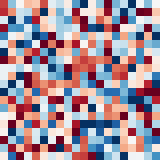
\includegraphics[width=0.32cm]{A}};
  \node[inner sep=0pt] at (0.2,0) {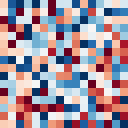
\includegraphics[width=0.32cm]{B}};
\end{scope}
\padlock[0.9]{4.77}{2.19}
% remote attestation icon: chip with shield
\begin{scope}[shift={(2.0,\sy)}]
  \foreach \j in {-0.2,-0.07,0.07,0.2}{\draw[dark,line width=0.55pt] (\j,0.3) -- (\j,0.4); \draw[dark,line width=0.55pt] (\j,-0.3) -- (\j,-0.4);
    \draw[dark,line width=0.55pt] (0.3,\j) -- (0.4,\j); \draw[dark,line width=0.55pt] (-0.3,\j) -- (-0.4,\j);}
  \fill[dark,rounded corners=1.2pt] (-0.3,-0.3) rectangle (0.3,0.3);
\end{scope}
\shield{2.0}{1.81}{teeC}
\foreach \a/\b in {16.6/15.5,14.5/13.4,12.4/11.3,10.3/9.12}
  \draw[fo] (\a,\sy) -- (\b,\sy);
\draw[fo] (8.25,\sy) -- (4.85,\sy);
\draw[fo] (2.45,\sy) -- (3.85,\sy);
% legend
\draw[f] (5.6,1.2) -- ++(0.5,0) node[right,lab]{Online inference};
\draw[fo] (5.6,0.85) -- ++(0.5,0) node[right,lab]{One-time setup};
% deployment arrows into the device
\draw[fo] (8.7,2.22) -- (8.7,2.38) -| (6.25,3.97);
\draw[fo] (4.35,2.16) -- (4.35,5.93);
% prediction back to client (bridged over setup arrows)
\draw[f,bridge] (17.125,3.42) -- (17.125,2.73) -- (0.975,2.73) -- (0.975,3.45);
\node[n] at (9.9,2.73) {6};
\end{tikzpicture}
\end{document}
